\documentclass[aspectratio=169,10pt]{beamer}
\usetheme{UniBern}
\title{Tomographic imaging of fish}
\subtitle{Or how to image much, \emph{much} more teeth}
\author{David Haberthür}
\institute{Institute of Anatomy\\Universität Bern}
\date{January 18, 2024, Institute Seminar}
\begin{document}

\begin{frame}
\maketitle
\end{frame}

\begin{frame}
	\frametitle{Grüessech mitenang!}
	\begin{itemize}
		\item David Haberthür
		\begin{itemize}
			\item Physicist by trade
			\item \href{https://boris.unibe.ch/2619/}{PhD in high resolution imaging of the lung}, Institute of Anatomy, University of Bern, Switzerland
			\item Post-Doc I: \href{https://www.psi.ch/sls/tomcat/}{TOMCAT}, \href{https://www.psi.ch/sls/}{Swiss Light Source}, \href{https://www.psi.ch/}{Paul Scherrer Institute}, Switzerland
			\item Post-Doc II: \uct{} group, Institute of Anatomy, University of Bern, Switzerland.
		\end{itemize}
	\end{itemize}
\end{frame}

\begin{frame}
	\frametitle{Grüessech from the \uct-group}
	\centering
	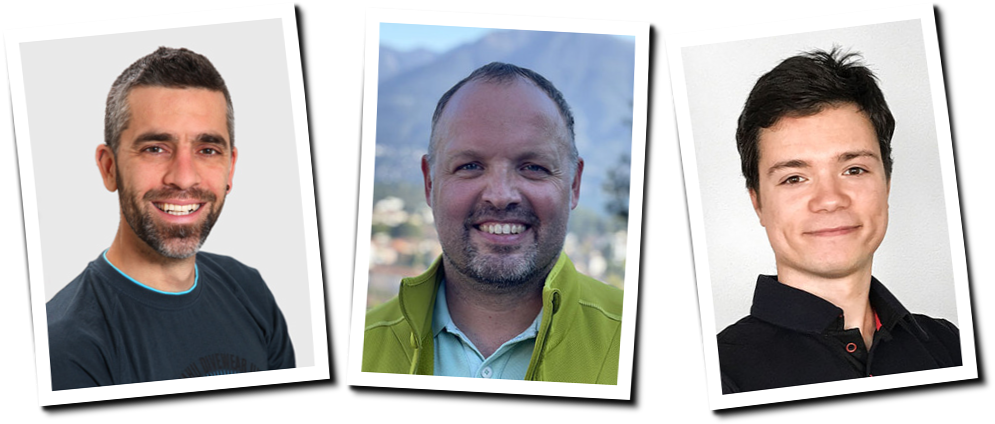
\includegraphics[height=\imageheight]{./images/team}
		\begin{columns}
		\hfill\begin{column}{0.33\textwidth}
			\centering%
			David{\color{ubRed!61.8}.}Haberthuer{\color{ubRed!61.8}@unibe.ch}%
		\end{column}
		\begin{column}{0.33\textwidth}
			\centering%
			Ruslan{\color{ubRed!61.8}.}Hlushchuk{\color{ubRed!61.8}@unibe.ch}%
		\end{column}
		\begin{column}{0.33\textwidth}
			\centering%
			Oleksiy{\color{ubRed!61.8}.}Khoma{\color{ubRed!61.8}@unibe.ch}%
		\end{column}\hfill%
	\end{columns}
\end{frame}

\renewcommand{\imagewidth}{\columnwidth}
\begin{frame}
	\frametitle{\uct-group}
	\begin{columns}
		\begin{column}{0.62\textwidth}
			\begin{itemize}
				\item microangioCT~\cite{Hlushchuk2018}
				\begin{itemize}
					\item Angiogenesis: heart, musculature~\cite{Nording2021} and bones
					\item Vasculature: (mouse) brain~\cite{Hlushchuk2020}, (human) nerve scaffolds~\cite{Wuthrich2020}, (human) skin flaps~\cite{Zubler2021} and tumors
				\end{itemize}
				\item Zebrafish musculature and gills~\cite{MesserliAaldijk2020}
				\item (Lung) tumor detection and metastasis classification~\cite{Trappetti2021}
				\item Collaborations with museums~\cite{Bochud2021} and scientist at UniBe~\cite{Halm2021,Kadlag2023} to scan a wide range of specimens, from human hearing bones to meteorites
				\item Automate \emph{all} the things!~\cite{Haberthuer2021,Haberthuer2023}
			\end{itemize}
		\end{column}%
		\begin{column}{0.38\textwidth}%
			\centering%
			\includegraphics<1|handout:0>[width=\imagewidth]{./images/1172}%
			\only<1|handout:0>{\source{brukersupport.com}{}}%
			\includegraphics<2|handout:1>[width=\imagewidth]{./images/1272}%
			\only<2|handout:1>{\source{bruker.com/skyscan1272}{}}%
			\includegraphics<3|handout:0>[width=\imagewidth]{./images/2214}%
			\only<3|handout:0>{\source{bruker.com/skyscan2214}{}}%
		\end{column}%
	\end{columns}%
\end{frame}

\begin{frame}[allowframebreaks]
	\frametitle{References}
	\renewcommand*{\bibfont}{\scriptsize}
	\setbeamertemplate{bibliography item}{\insertbiblabel}
	\printbibliography{}
\end{frame}

\end{document}
